\documentclass{article}

\usepackage{graphicx}
\usepackage{float}
\usepackage{caption}
\usepackage{subcaption}

\pagestyle{empty}

\begin{document}

%% PANEL 1
\begin{figure}
  \begin{subfigure}[b]{\textwidth}
    \caption{}
    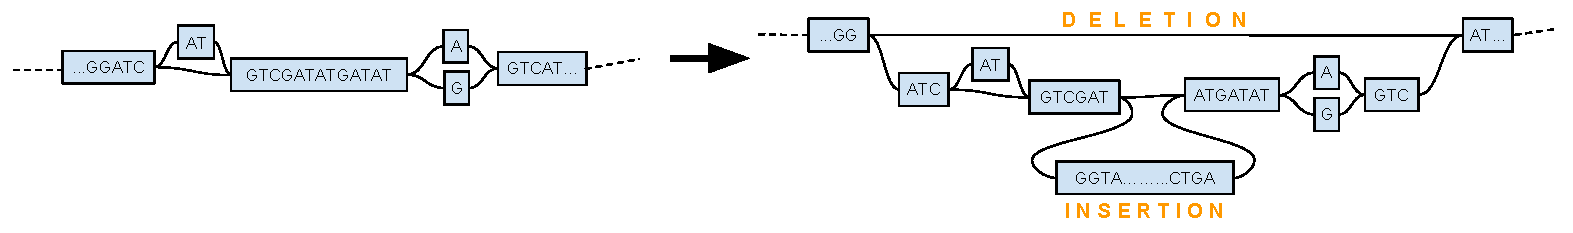
\includegraphics[width=\textwidth]{pdf/VGSVcartoon.pdf}
  \end{subfigure}

  \begin{subfigure}[b]{\textwidth}
    \caption{}
    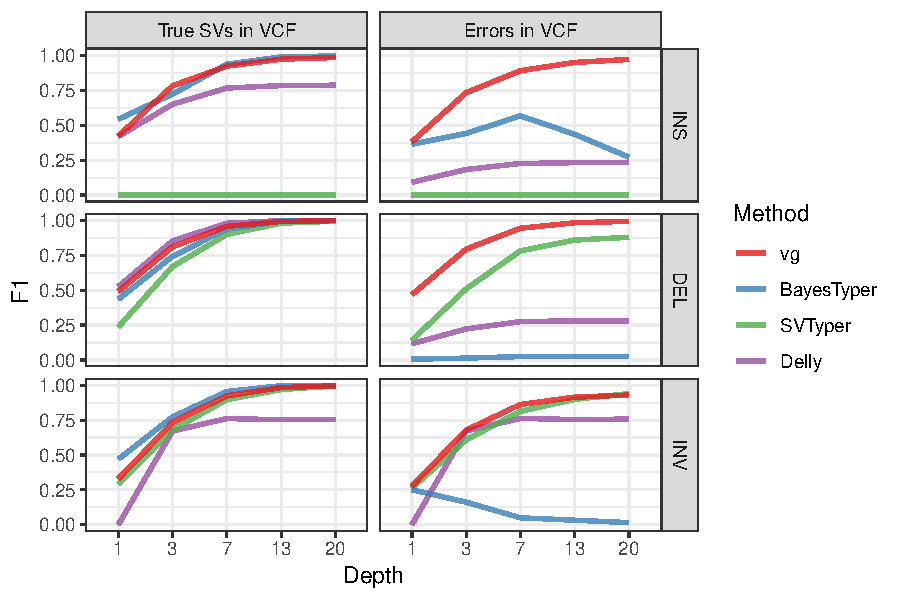
\includegraphics[width=\textwidth]{pdf/simerror-geno.pdf}
  \end{subfigure}
\end{figure}

%% PANEL 2
\clearpage
\begin{figure}
  \begin{subfigure}[b]{\textwidth}
    \caption{}
    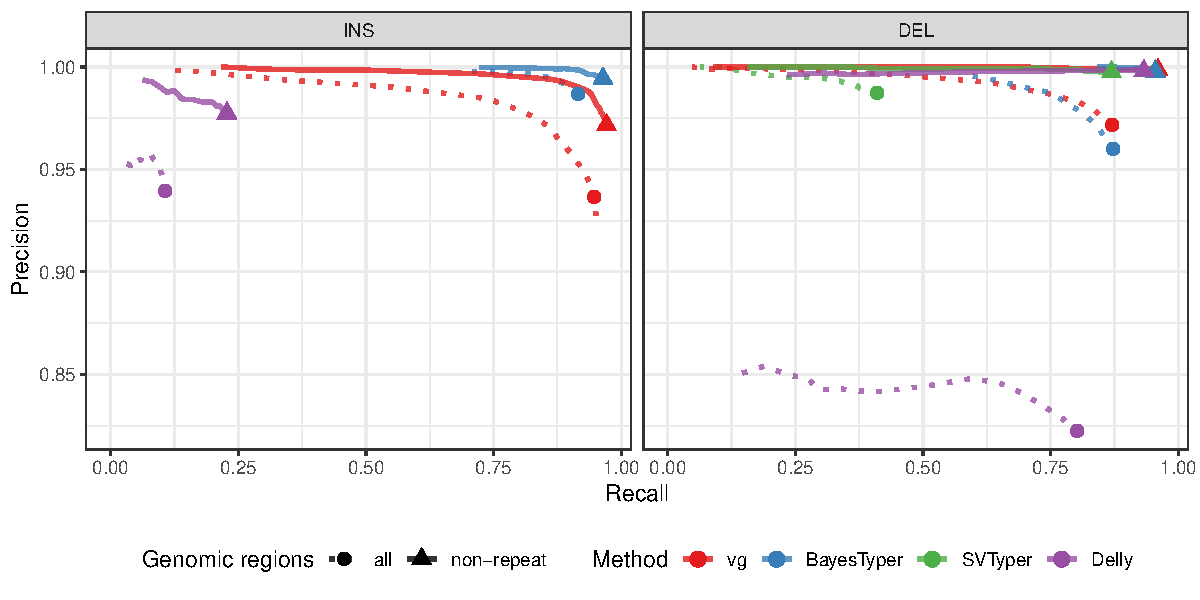
\includegraphics[width=\textwidth]{pdf/hgsvc-sim.pdf}
  \end{subfigure}

  \begin{subfigure}[b]{\textwidth}
    \caption{}
    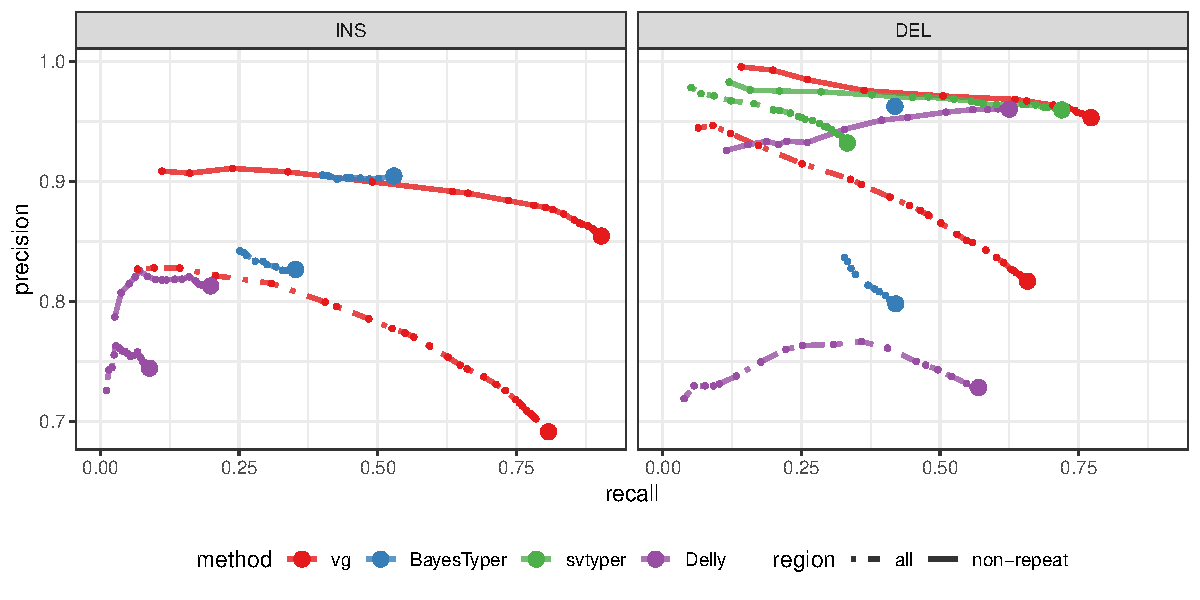
\includegraphics[width=\textwidth]{pdf/hgsvc-real.pdf}
  \end{subfigure}
\end{figure}

%% PANEL 3
\clearpage
\begin{figure}
  \begin{subfigure}[b]{.5\textwidth}
    \caption{}
    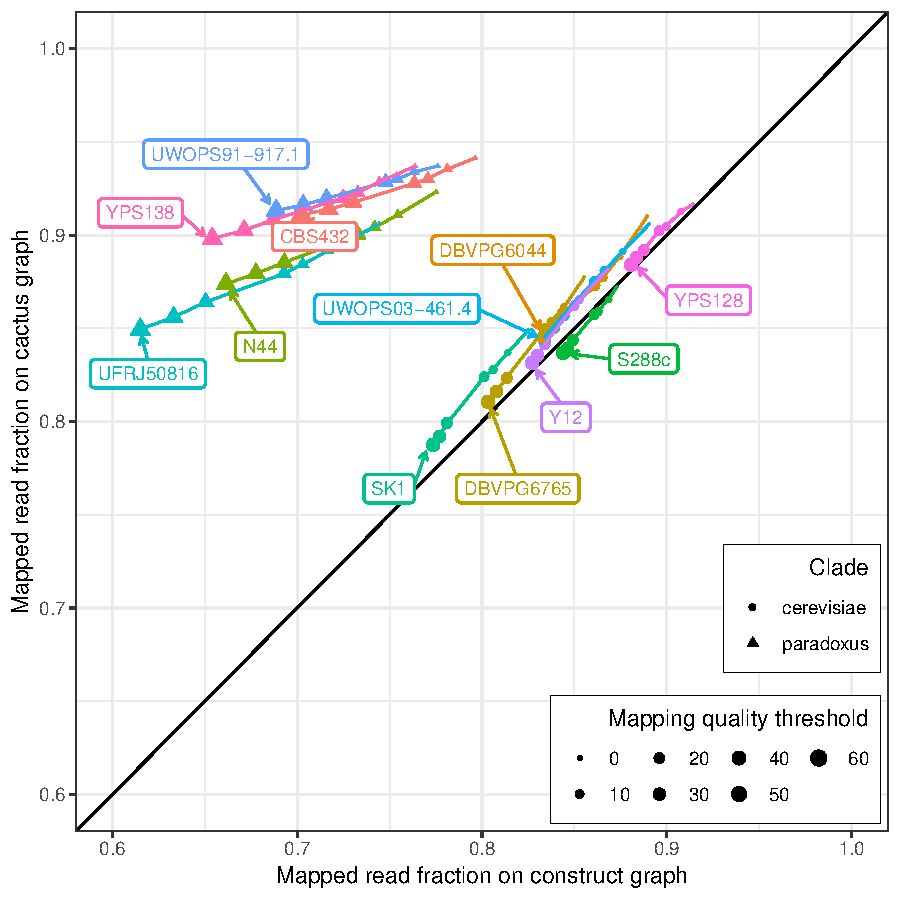
\includegraphics[width=\textwidth]{pdf/yeast-mapping-quality-all.pdf}
  \end{subfigure}
  \begin{subfigure}[b]{.5\textwidth}
    \caption{}
    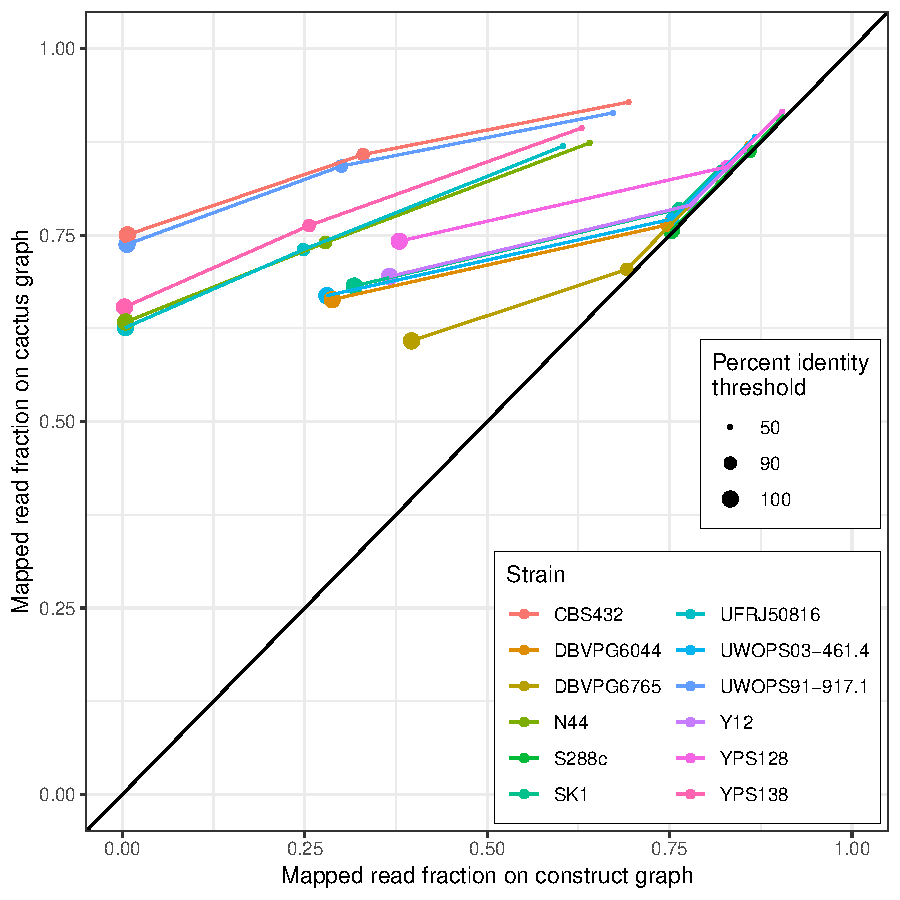
\includegraphics[width=\textwidth]{pdf/yeast-mapping-identity-all.pdf}
  \end{subfigure}
\end{figure}

%% PANEL 4
\clearpage
\begin{figure}
  \begin{subfigure}[b]{.5\textwidth}
    \caption{}
    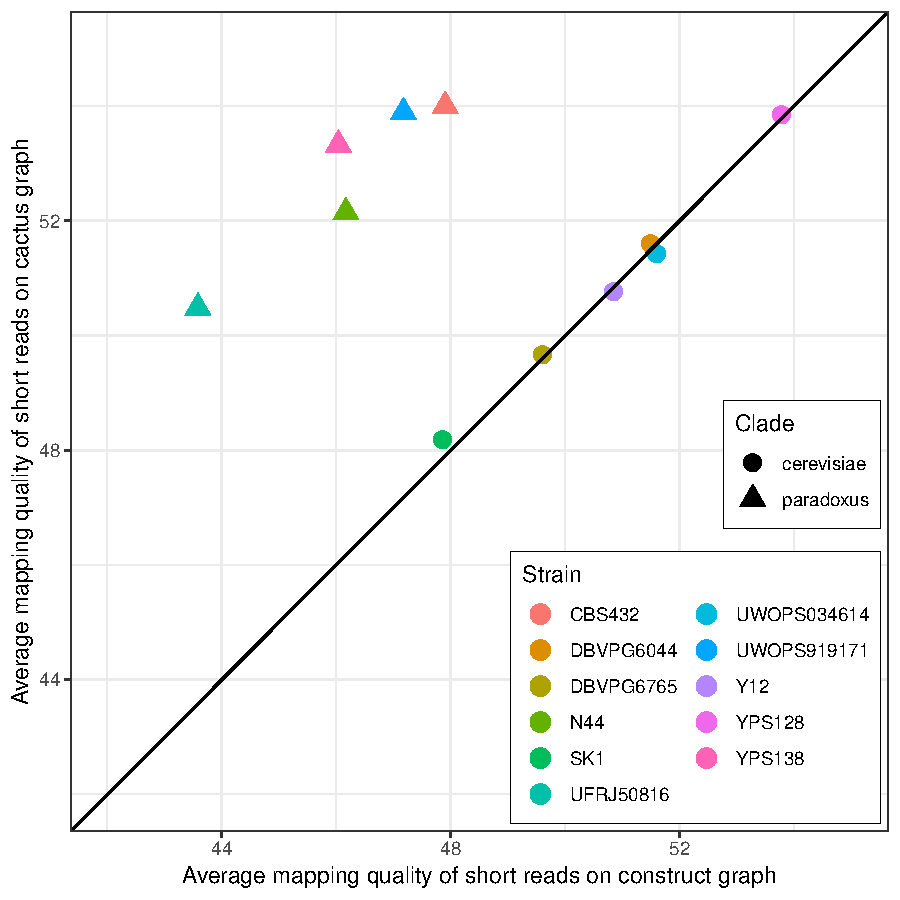
\includegraphics[width=\textwidth]{pdf/yeast-genotyping-quality.pdf}
  \end{subfigure}
  \begin{subfigure}[b]{.5\textwidth}
    \caption{}
    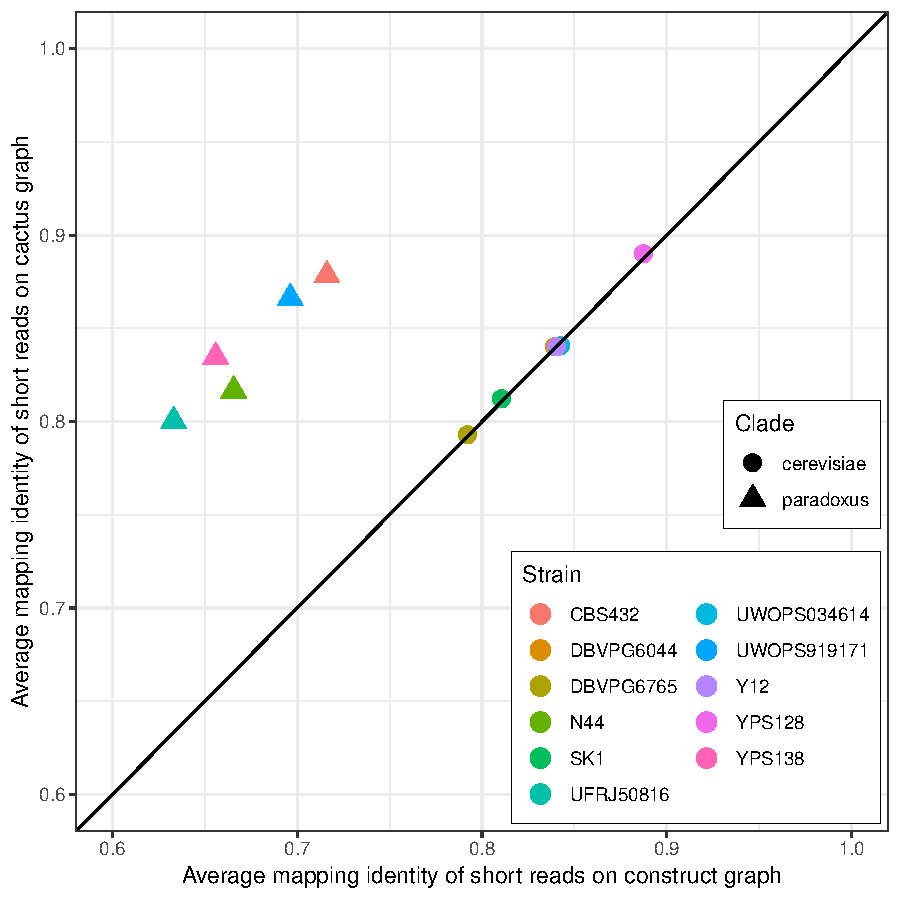
\includegraphics[width=\textwidth]{pdf/yeast-genotyping-identity.pdf}
  \end{subfigure}
\end{figure}

%% PANEL 5 (Supplementary)
\clearpage
\begin{figure}
  \begin{subfigure}[b]{.5\textwidth}
    \caption{}
    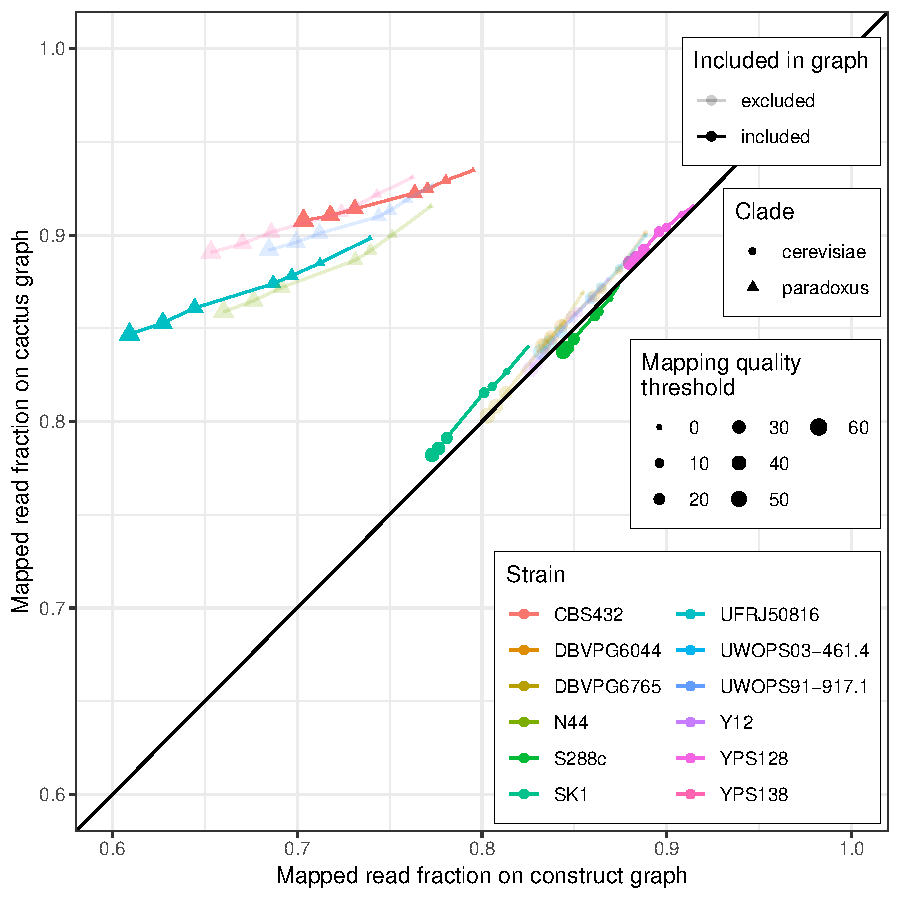
\includegraphics[width=\textwidth]{pdf/yeast-mapping-quality-four.pdf}
  \end{subfigure}
  \begin{subfigure}[b]{.5\textwidth}
    \caption{}
    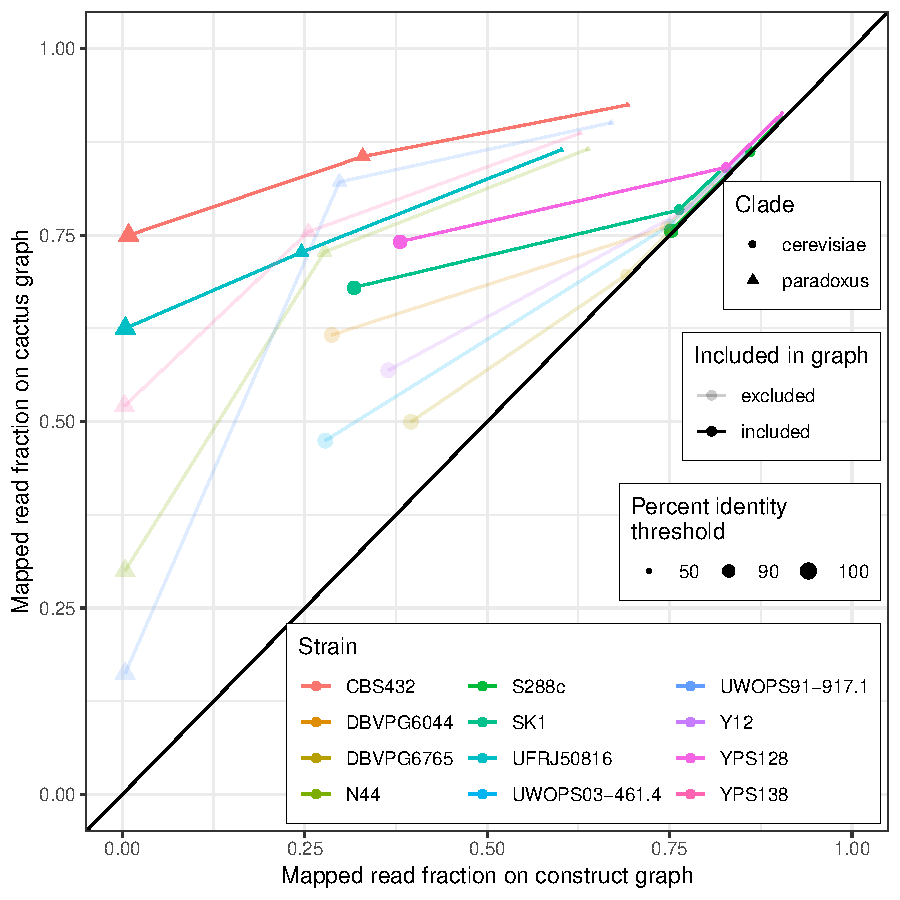
\includegraphics[width=\textwidth]{pdf/yeast-mapping-identity-four.pdf}
  \end{subfigure}
\end{figure}

\end{document}



%%% Local Variables:
%%% mode: latex
%%% TeX-master: t
%%% End:
